

\chapter{关键词检测的序列建模和标签同步解码}
\label{chap:kws}

语音识别是一种序列预测问题。除了需要研究如何将各种基于深度学习的模型方法应用到逐帧分类当中,使用序列级的鉴别性训练准则来强化模型的序列分类能力,也被证明是取得业界最好的大词汇连续语音识别系统的关键。但是关键词检测(KWS), 作为语言识别最主要的应用之一,几乎只受到了逐帧训练的深度学习的改善,却少有研究解决其鉴别性训练问题。这里的主要原因来自鉴别性训练中的归一化项在KWS任务中不容易建模。
有少数研究尝试这一方向,但集中在固定关键词表的关键词检测或者基于LVCSR的关键词检测,并且它们也没有与当前主流的深度学习方法相结合。
在本章中,我们提出了针对固定或者非固定关键词的关键词检测系统的序列鉴别性训练框架。我们系统地研究了序列生成模型和序列鉴别模型情况下的序列鉴别性训练
通过引入词语无关的音素词图或非关键词的 {\em blank} 单元来构建竞争性搜索空间,我们在声学KWS系统上提出了一系列有效并且高效的序列鉴别性训练方法 。使用表明我们提出的方法取得了一致并且显著的改善。测试包括固定关键词或非固定关键词的关键词检测任务,比较的基线是逐帧的深度学习声学KWS模型方法。

\section{引言}\label{Sec:kws-intro}

%KWS
%method categorized, what we discuss

关键词检测(KWS)是语言识别最主要的应用之一,它的目标是得到一个高准确度和高效率的识别器,用于检测特定的一些关键词在语音中的出现。
KWS可以被用于声学数据挖掘~\cite{zhou2005data}, 低资源的音频检索~\cite{shen2009comparison}, 
语料库检索~\cite{garofolo2000trec} 和 唤醒词识别~\cite{chen2014small}. 本文主要考虑后两种应用。


KWS 技术可以被分为两大类:
i) 非监督的  {\em query-by-example} (QbyE) \cite{zhang2009unsupervised,barakat2012improved,chen2015query}, 它使用了关键词的声学样例来产生一系列模板,之后尝试将模板与测试音频样例进行匹配来决定是否被唤醒。
ii) 监督的基于文本的方法,这部分可以被进一步分类为  基于{\em 大词汇连续语音识别} (LVCSR)  方法 ~\cite{garofolo2000trec,ng2000subword} 和  {\em 声学 KWS} \cite{mandal2014recent}。
对于前者,在训练阶段需要构建一个词,半词或音素的语音识别系统。声学和语言模型在测试阶段一起对语音进行转录并得到词图。之后在词图上进行关键词搜索得到最终的结果。
声学 KWS 不需要语言模型,通过直接建模目标关键词,半词或音素,构建一个声学模型来进行关键词的判别。一些方法中也会考虑引入非关键词元素到建模当中~\cite{sukkar1996utterance}。
QbyE 主要用于低资源音频检索, 本文不针对这个方向。 
在 语料库检索中, 基于LVCSR方法通常能得到更好的性能,相比声学KWS。但是基于LVCSR方法也有如下一些缺点: 需要训练一个非常通用的大词汇连续语音识别系统,因此需要大量语料;同时在测试阶段也需要非常大的词表进行覆盖。这样的缺点限制了它在一些应用,比如唤醒词识别,中的应用。除此之外,基于LVCSR的方法忽略了KWS任务本身的一些特性,改进这类方法主要跟改进大词汇连续语音识别声学建模相关。所以本章节主要研究声学KWS。

在声学关键词检测中,模型通常是进行逐帧分类的。目前研究趋势包括两方面:应用一个较强的逐帧分类器,比如深度学习模型,使最终系统带来性能提升~\cite{chen2014small,sainath2015convolutional}。 其次,语音识别本身是一个序列分类问题,传统的GMM-HMM系统在使用序列级准则,序列鉴别性训练时,往往能带来显著性能提升,比如discriminatively trained sub-word verification function~\cite{sukkar1996vocabulary}, minimum classification error (MCE)~\cite{sandness2000keyword} 和 performance-related discriminative training~\cite{keshet2009discriminative}。
在上述的鉴别性训练中,对对识别可能性的建模,即完整的搜索空间的建模是成功的关键。但是,在 KWS中,由关键词所定义的领域内搜索空间要显著小于领域外的搜索空间。因此领域外的搜索空间通常还需要特定的建模单元进行建模。
对领域外的搜素空间建模并不容易直接得到的问题限制了序列鉴别性训练在关键词检测中的广泛应用。
特别是在非固定关键词的关键词检测, 所以可能的竞争可能性通常无法被穷举,同时这种可能性的产生过程在使用LVCSR框架进行的时候~\cite{povey2005discriminative}非常耗时。 
%combination of both hasn't been carefully 

%Neural networks (NNs) for speech recognition are typically trained to classify individual frames based on a cross-entropy criterion (section 2.1).
在这篇文章中,我们为深度学习的 声学非固定关键词的关键词检测设计了相应的序列鉴别性训练方法。关于如何对序列概率进行定义,可分为序列条件似然度和序列后验概率,这包括两种序列模型: {\em 生成式序列模型} (GSM),比如HMM, 和 {\em 鉴别式序列模型} (DSM),比如 CTC。
对于GSM,序列鉴别性训练需要在序列上使用贝叶斯公式来通过序列条件似然度得到后验概率;而DSM则可以直接使用序列后验概率。

对这两种框架,竞争可能性的建模都是核心难题。本章节提出两种方法来解决这一问题:隐性使用音素或半词单元的语言模型来建模,或者显性加入非关键词的标签。
%proposed KWS 
%Both frameworks are improved in the paper. 
在HMM中,受到近期一些研究中使用特点音素语言模型来对LVCSR的搜索空间进行建模的启发~\cite{povey2016purely,chen2006advances},  我们提出使用这种音素语言模型来对关键词的完整搜索空间进行建模。
为了加强关键词的鉴别能力,在关键词出现时候它们的梯度可以被增强。除此之外,许多神经网络结构和鉴别性训练准则也进行了详细比较。
在CTC中,非关键词建模单元被直接引入到建模当中。具体来说,加入之后的CTC模型搜索空间包括了关键词,音素边界 ($\tt blank$) 和词边界 ($\tt wb$)。 
最后我们基于前面章节介绍的LSD算法提出了一种高效的后处理算法,以解决音素混淆建模的问题。

本章节的主要贡献包括:
i) 针对生成式序列模型和鉴别式序列模型的序列鉴别性训练的第一个系统研究工作
ii) 提出了一些新颖的办法来构建声学KWS的竞争可能性,以用于鉴别性训练。这些方法显著提升了关键词检测系统的性能。
iii) 基于 LSD框架提出了高效的后处理方法,以便对音素混淆性进行建模。

\section{关键词检测的声学建模}
\label{Sec:kws-and-disc}

基于声学的关键词检测模型通常是要最小化每一帧的分类错误。在深度学习的HMM混合系统 (NN-HMM) 中,使用的是 tri-phone state作为建模单元,而深度学习模型则用来对每个HMM状态的后验概率进行建模。
特别是,对特征输入 ${\bf o}_{ut}$ 关于时间 $t$ 在句子 $u$中, 定义 $y_{ut}(s)=P(s|{\bf o}_{ut})$ ,表示神经网络在HMM 状态 $s$上的相应输出。这里的公式类似于GMM-HMM 系统~\cite{young1994state}, 除了需要使用伪对数似然度 $\log p({\bf o}_{ut}|s)$ 来针对HMM状态 $s$。
\begin{equation}
\label{equ:dnn-hmm-define}
\begin{split}
 p({\bf o}_{ut}|s) \propto \frac{ y_{ut}(s)}{ P(s)}
\end{split}
\end{equation}
公式中 $P(s)$ 是状态 $s$的先验概率。 
在深度学习系统中,如果建模单元是关键词,那么关键词 $w$ 的后验概率是要被直接训练得到的:
\begin{equation}
\label{equ:dnn-kw-define}
\begin{split}
P(w|{\bf o}_{ut})= y_{ut}(w)
\end{split}
\end{equation}
而前面讨论的后处理方法要被应用于逐帧的后验概率$y_{ut}(w)$上面。

%CE formula
这里通常可以使用负对数后验概率来作为交叉熵的目标函数。
\begin{equation}
\label{equ:dnn-hmm-ce}
\begin{split}
\mathcal{F}_{\tt{CE}}=- \sum_{u} \sum_{t} \log y_{ut}(s^{(r)}_{ut})
\end{split}
\end{equation}
公式中 $s^{(r)}_{ut}$ 是在时间 $t$ 句子 $u$ 上的标注,通过状态级强制对齐算法来得到~\cite{woodland1994large}。


\section{序列鉴别性训练}
\label{Sec:sdt-review}
由于语音识别本身是一个序列预测问题,所以序列级的准则往往能够带来性能的提升。依据序列的不同定义方式,目前有两种不同的序列鉴别性训练方法,一种针对  生成式序列模型 (GSM) 比如HMM,另一种针对 鉴别式序列模型 (DSM) ,比如 CTC 或者 encoder-decoder 模型。 
%序列鉴别性训练 for GSM is discussed in Section~\ref{Sec:sgm-sdt-intro} and DSM based 序列鉴别性训练 is discussed in Section~\ref{Sec:sdm-sdt-intro}.
 %while 序列鉴别性训练 in  CTC framework is considered in Section~\ref{Sec:kws-ctc}.

%table to show 
%       frame seq
%gen
%disc


\subsection{生成式序列模型 和 鉴别式序列模型 在ASR中的应用}
\label{Sec:sgm-and-sdm}
在语音识别中一个独有并且有趣的自然现象是声学序列和语言学序列的长度可变性。
序列模型正是被提出用来解决两个序列之间的关联性。大部分序列模型都包含一个用来对时序特性建模的部分, 比如GMM~\cite{woodland1994large} 和深度学习模型~\cite{hinton2012deep}用来对局部的声学特征进行建模,再加上一个对序列长度和转移进行建模的部分,比如HMM。近期提出的鉴别式序列模型, encoder-decoder~\cite{chan2016end}则尝试直接对序列建模而不是进行序列到逐帧的拆分。但在KWS中,性能和延迟在上述模型中都有一定限制。因此不参与本章节讨论。
本章节所有的序列鉴别性训练方法均基于逐帧的分解方式。基于模型是对条件似然度或者后验概率进行建模,概率模型通常可以分为生成式和鉴别式两种类型。值得注意的是在序列上或者在帧上,都可以使用生成式或者鉴别式进行分别建模,二者工作在不同层面上。
比如目前通常使用的混合 NN-HMM 模型就是采用生成式序列模型和鉴别式帧分类器。
在本章节中,我们主要关注序列模型。下文我们将比较模型结构和优化准则,在生成式和鉴别式序列模型中的异同。

 %There are two branches of sequence models. 生成式序列模型 is to model $P(\mathbf{O}|\mathbf{L})$ and 鉴别式序列模型 is to model $P(\mathbf{L}|\mathbf{O})$.

{\em 生成式序列模型}通常被定义为条件似然度$p(\mathbf{O}|\mathbf{L})$, 公式中 ${\mathbf O}$ 表示特征输入序列, $\mathbf L$ 表示标签输出序列。隐马尔可夫模型 (HMM) 是这类生成式序列模型的一个经典例子~\footnote{另一类 GSM 例子是Kalman 滤波器~\cite{digalakis1991dynamical,abbeel2005discriminative}.}. 
在NN-HMM 混合系统中, 语音信号的动态性使用HMMs 和来自深度学习模型的后验概率进行建模。
\begin{eqnarray}
\label{equ:hmm-model_2}
%\begin{split}
p(\mathbf{O}|\mathbf{L})&=&\!\!\!\!\!\!\sum_{\mathbf{q}\in\mathcal{A}(\mathbf{L})}\!\!\!p(\mathbf{O},\mathbf{q}|{\mathbf L}) =\sum_{\mathbf{q}}\prod_{t=1}^{T} p({\bf o}_{t}|q_t) P(q_t|q_{t-1})\nonumber\\
%y_{ut}(s^{(r)}_{ut})
&\propto&\sum_{\mathbf{q}}\prod_{t=1}^{T} \frac{P(q_t|{\bf o}_{t})}{P(q_t)}P(q_t|q_{t-1})
%\end{split}
\end{eqnarray}
公式中 $\mathbf{L}$ 表示标签序列,比如LVCSR中的词序列。
$\mathbf{q}$ 表示HMM状态序列,  $q_t$ 表示在帧 $t$上的HMM状态序列。 $P(q_t|q_{t-1})$ 表示 HMM 状态转移概率, $P(q_t)$表示状态的先验概率。
$\mathcal{A}$表示由标签序列 $\mathbf{L}$到它的相应HMM状态序列 $\mathbf{q}$之间的映射,
\begin{equation}
\label{equ:a-func_2}
\begin{split}
\mathcal{A}:\mathbb{L}  \mapsto \{ q_0^{(1)},\cdots,q_4^{(1)},\cdots,q_4^{(|\mathbb{L}|)} \}
\end{split}
\end{equation}
$\mathbb{L}$ 表示 $\mathbf{L}$中所有的标签。 $q_s^{(l)}$ 表示第l个HMM的第s个 HMM 状态。
具体来说,每个标签单元,比如 tri-phone, 对应于一个 HMM 模型。
每个HMM模型则包含5个独立的状态,如图~\ref{fig:hmm-topo}(a)所示。
状态后验概率 $P(q_t|{\bf o}_{ut})$是由神经网络来估计得到的。
当一个序列级鉴别性训练准则,比如序列后验概率,被优化时,我们一般采用贝叶斯公式分解来使得生成式模型可以使用鉴别性准则进行优化。



{\em 鉴别式序列模型} 由 $P(\mathbf{L}|\mathbf{O})$进行定义,表示给定特征序列$\mathbf{O}$建模序列 $\mathbf{L}$的后验概率。 
连接时序模型 (CTC)~\cite{graves2006connectionist} 是其中一种鉴别式序列模型. 它引入了 $\tt blank$标签来建模输出标签之间的混淆部分。具体来说,这种模型会在两个标签$l_{i-1}$ 和 $l_{i}$之间预测出 $ \tt blank$ 建模单元。
公式中的 $\mathcal{B}$ 是一个一对多的映射函数~\footnote{在最早文献~\cite{graves2006connectionist}中使用的公式定义为一个多对一的映射函数,同时使用它的反函数来定义 $\mathcal{B}^{-1}(\cdot)$ CTC模型中的映射。这里我们修改为一个一对多的映射函数,使公式与HMM中的定义更加一致。}:
\begin{equation}
\label{equ:ctc-b_2}
\begin{split}
\mathcal{B}:\mathbb{L}   \mapsto  \mathbb{L} \cup \{\tt blank\}
\end{split}
\end{equation}
$\mathcal{B}$ 决定了标签序列 $\mathbf{L}$ 和它相应的由建模单元所组成的模型状态序列$\mathbf{q}$。 这一映射的做法是在每个组成 $\mathbf{L}$ 的$l$的标签中,插入一个可选的并且可重复的 $ \tt blank$ 标签。 $P(q_t|\mathbf{O})$是由深度学习模型直接根据给定的特征序列$\mathbf{O}$来估计得出的, 比如使用LSTM~\cite{hochreiter1997long}。 
当使用了序列鉴别性模型之后,序列鉴别性准则的优化形式就非常直接。

%In summary, sequence models are used to model the temporal characteristics of the acoustic feature sequences. 
%
%They can be divided into 生成式序列模型 and 鉴别式序列模型. 
%Further investigations are given  in Section~\ref{Sec:disc-and-ctc}.

\subsection{基于HMM的序列鉴别性训练}
\label{Sec:sgm-sdt-intro}

使用隐马尔科夫模型 (HMM), 在进行序列鉴别性训练之前,需要首先使用贝叶斯公式计算序列后验概率。
\begin{equation}
\label{equ:map-dec}
\begin{split}
P(\mathbf{W}_u|\mathbf{O}_u)=\frac {p(\mathbf{O}_u|\mathbf{W}_u)P(\mathbf{W}_u)}{p(\mathbf{O}_u)}  
%y_{ut}(s^{(r)}_{ut})
\end{split}
\end{equation}
公式中$\mathbf{W}_u$ 是句子 $u$ 对应的词序列。 $P(\mathbf{W}_u)$ 是语言模型概率。在KWS中,$P(\mathbf{W}_u)$ 被定义为关键词和非关键词序列的先验概率。
$p(\mathbf{O}|\mathbf{W})$ 是相应的声学部分,由下式得到。
%INTRO: W relation with L
\begin{equation}
\label{equ:lexicon}
\begin{split}
p(\mathbf{O}|\mathbf{W})=\sum_{\mathbf{L}\in\mathcal{L}(\mathbf{W})} p(\mathbf{O}|\mathbf{L})P(\mathbf{L}|\mathbf{W})
%y_{ut}(s^{(r)}_{ut})
\end{split}
\end{equation}
公式中 $p(\mathbf{O}|\mathbf{L})$ 是由HMM中的定义公式(\ref{equ:hmm-model_2})给定的。 $\mathcal{L}$定义了从词序列 $\mathbf{W}$ 到它的标签序列 $\mathbf{L}$ 的映射, 比如LVCSR中的tri-phone 序列。 $P(\mathbf{L}|\mathbf{W})$ 是发音概率~\cite{chen2015pronunciation} 通常由词典和语言模型来决定。

特征序列 $\mathbf{O}_u$ 的边缘概率 $p(\mathbf{O})$是由所有可能的序列的概率进行求和得到的。
\begin{equation}
\label{equ:po-prob}
\begin{split}
p(\mathbf{O}_u)=\sum_\mathbf{W} p(\mathbf{O}_u,\mathbf{W})= \sum_\mathbf{W} P(\mathbf{W}) p(\mathbf{O}_u|\mathbf{W})
%y_{ut}(s^{(r)}_{ut})
\end{split}
\end{equation}
公式中 $\mathbf{W}$ 表示其中一条竞争的可能路径,具体来说是词图中的一条解码路径。
作为序列鉴别性训练的一个例子,最大互信息准则 maximum mutual information (MMI)~\cite{bahl1986maximum} 如下定义,
%discriminative training formula (P(O) traditional)
\begin{equation}
\label{equ:lvcsr-mmi}
\begin{split}
\mathcal{F}_{\tt{MMI}}%=\sum_{u} \log P(\mathbf{W}_u|\mathbf{O}_u)\\
%=- \sum_{u} \log \frac {p(\mathbf{O}_u|\mathbf{S}_u)^{\kappa}P(\mathbf{W}_u)}{\sum_{\mathbf{W}} p(\mathbf{O}_u|\mathbf{S})^{\kappa}P(\mathbf{W})}  
=\sum_{u} \log \frac {p(\mathbf{O}_u|\mathbf{W}_u)^{\kappa}P(\mathbf{W}_u)}{\sum_{\mathbf{W}} p(\mathbf{O}_u|\mathbf{W})^{\kappa}P(\mathbf{W})}  
\end{split}
\end{equation}
公式中的分布 $P(\mathbf{W}_u|\mathbf{O}_u)$, 在 (\ref{equ:map-dec})中, 由一个常量 $\kappa$ 进行调节。 %$\mathbf{S}$ and $\mathbf{S}_u$ is the acoustic model state sequences corresponding to $\mathbf{W}$ and $\mathbf{W}_u$ respectively. 
在公式(\ref{equ:lvcsr-mmi})中给定了序列后验概率表达式, 而其他一些序列鉴别性训练准则则是由贝叶斯风险框架推导得到的,将在接下来的章节中进行讨论~\ref{Sec:lfmmi-train}。

基于深度学习的LVCSR和基于LVCSR的KWS都可以被序列鉴别性准则所改进~\cite{vesely2013sequence,meng2016non}. 
%the key is use LATTICE 
这里的序列竞争可能路径 $\mathbf{W}$ 在 (\ref{equ:po-prob})中可以从,与语言模型一起进行联合解码,而得到。解码得到的词图作为一种搜索空间的紧致表示,可以用于计算公式(\ref{equ:po-prob})中的边缘概率 $p(\mathbf{O}_u)$ 。

  
%traditional GMM-HMM based systems achieve significantly better performance when trained using sequence discriminative criteria like WB-MVE~\cite{sukkar1996utterance},  discriminatively trained sub-word verification function~\cite{sukkar1996vocabulary}, MCE~\cite{sandness2000keyword} and performance-related discriminative training~\cite{keshet2009discriminative}.
在声学KWS方法中,只有关键词序列被定义,而非关键词的竞争序列还未知。基于似然度比值的可能性测试框架~\cite{sukkar1996utterance} 被提出以进行鉴别性训练,这里对其他竞争序列的似然度进行了惩罚。而这部分被惩罚的似然度使用两种单元进行建模: $\tt filler$ 模型, 建模非关键词的$p(\mathbf{O}_u|\Phi)$, 建模错误识别词的 $p(\mathbf{O}_u|\Psi)$ 。 与公式~(\ref{equ:lvcsr-mmi})相比,关键词序列的  $p(\mathbf{O}_u|\mathbf{W}_u)$ 可以被忽略,而对数边缘概率则被定义如下,
\begin{equation}
\label{equ:wbmve-po}
\begin{split}
\log p(\mathbf{O}_u)=\left\{\frac{1}{2}[\log p(\mathbf{O}_u|\Psi)^\lambda + \log p(\mathbf{O}_u|\Phi)^\lambda]\right\}^{1/\lambda}
%y_{ut}(s^{(r)}_{ut})
\end{split}
\end{equation}
这里的序列竞争可能序列 $\mathbf{W}$ 是由N-best序列得到的。
%In~\cite{sukkar1996vocabulary},
在这些方法中,人工加入的非关键词单元并不能进行很好的建模,原因是发音和声学的不同并没有办法完全囊括在一个建模单元当中。除此之外,该方法也没有对关键词和非关键词之间的上下文进行建模。另外由N-best得到竞争序列也并不重复。最后,该类方法也无法应用到非固定关键词的关键词检测中。

\subsection{CTC based 序列鉴别性训练}
\label{Sec:sdm-sdt-intro}
%discriminate KW or discriminate KW \& filler, but filler is imperfect

{\em{鉴别式序列模型}} 是直接对序列后验概率进行估计的一类模型,如公式 (\ref{equ:ctc-model})所示。
连接时序模型 (CTC) 是一个典型的例子~\cite{graves2006connectionist,huang2018ctc}。
在~\cite{fernandez2007application}中, CTC被应用到KWS中。
CTC的输出被定义为所有可能的关键词序列 $\mathbf{W}$的后验概率。其目标函数是:
\begin{equation}
\label{equ:ctc-formu}
\begin{split}
\mathcal{F}_{\tt{CTC}}=\sum_{u} \log P(\mathbf{W}_u|\mathbf{O}_u)\\
=\sum_{u} \log \sum_{\mathbf{L}\in\mathcal{L}(\mathbf{W}_u)} P(\mathbf{L}|\mathbf{O}_u)P(\mathbf{W}_u|\mathbf{L})
\end{split}
\end{equation}
公式中 $\mathbf{L}$ 是CTC模型的标签序列,比如半词或者音素序列等。
在声学KWS中,没有引入语言模型。 $P(\mathbf{W}_u|\mathbf{L})$ 是一个确定性的由词典到关键词序列的映射。
$P(\mathbf{L}|\mathbf{O}_u)$ 可以进一步映射到CTC模型的标签序列,并分解到每一帧如公式 (\ref{equ:ctc-model})所示。
注意到一个额外的$\tt blank$ 单元被引入到逐帧的公式 (\ref{equ:ctc-model})中以建模语音信号的混淆区段。
%
序列鉴别性准则定义为所有可能的CTC标签序列的概率求和,作为最终的优化方向。

在词级CTC~\cite{fernandez2007application}中, 
虽然它是一个序列级准则,但是并没有对非关键词部分进行建模。因此该准则改善了关键词之间的鉴别性,但是没有改善关键词和非关键词之间的鉴别性。


\section{基于HMM的关键词检测的序列鉴别性训练}
\label{Sec:kws-disc-proposed}

如前面的章节~\ref{Sec:sgm-sdt-intro}所述,将基于HMM的KWS使用序列鉴别性训练进行改善的主要难度在于如何得到词级别的可靠竞争序列估计。
受到之前研究中使用一个裁剪过的音素语言模型来代替词图在鉴别性训练中的应用的启发(称为 {\em 无词图鉴别性训练} (LF-MMI)~\cite{povey2016purely,chen2006advances}), 我们提出了一种通用的序列鉴别性训练框架,并针对非固定关键词的关键词检测任务。
这里的关键词序列由音素声学模型进行建模。相应我们就使用音素的语言模型来构建一个完整的搜索空间 ,使之包含关键词和非关键词的竞争序列。

\subsection{模型训练}
\label{Sec:lfmmi-train}

在所提出的音素声学模型中, (\ref{equ:lvcsr-mmi}) 被转换为 (\ref{equ:kws-mmi}) 并表示为 $\tt{LF\text{-}MMI}$。
公式中 $\mathbf{L}$ 是音素序列。 $\mathbf{L}_u$ 是标注标签序列。
$p(\mathbf{O}_u|\mathbf{L})$ 和 $p(\mathbf{O}_u|\mathbf{L}_u)$ 由公式~(\ref{equ:hmm-model_2})得到。 


该方法与传统鉴别性训练不同之处在于: 
\begin{itemize}
\item 在分母式子中所使用的标注序列 $\mathbf{L}_u$ 存在多种候选路径,这些候选路径来自于标注软对齐中对标签在一定窗宽内的左右帧移。这里将所有可能的对齐路径都存储在分子词图中。
\item 模拟搜索空间的分母语言模型 $P(\mathbf{L})$, $P(\mathbf{L}_u)$是使用一个在训练标注文本中训练得到的音素语言模型。
\item 一个专用的HMM拓扑结构被专门提出,它包含有两个HMM状态。其中状态${\bf q}_2$ 用于模拟CTC中的$\tt blank$ 建模单元,同时其他状态来模拟输出标签单元。这里的不同之处在于每个 tri-phone都维护一个它专有的$\tt blank$建模。
\item 输出帧率被降低了3倍。
\end{itemize}


%iv) the cross-entropy regularization is applied with moderately larger weight in the cross-entropy. The reason is that the sub-word level language model is unavailable in test stage. Empirically the model should balance between sequence level and frame level criteria.
%regu is similar but MTL-ce  


%model unit, hmm topo, state binding
为了更好地将 $\tt{LF\text{-}MMI}$ 应用到关键词检测当中,我们进行了如下改进:
i) 我们使用音素而不是tri-phone作为建模单元。
% to improve model inference efficiency. 
首先是在测试阶段,效率将会得到改善;其次是这样会使得后文将讨论的 $\tt filler$ 构建显著简化。
ii) HMM的拓扑结构如图~\ref{fig:hmm-topo}(d-e)所示进行了修改,
本文将图\ref{fig:hmm-topo}(d-e)所示的几种改进的HMM拓扑结构应用在了GSM中。具体来讲,在图\ref{fig:hmm-topo}(c)中,每个CD音素都有独立的blank状态,称为CD音素blank (CD phone blank)。为减少模型单元的数量并进一步加快算法速度,将中心音素相同的blank状态绑定在一起,称为音素级blank (phone blank);最后如果绑定所有的blank状态则称作全局blank (global blank)。此外,鉴于标签延迟带来的性能改进\cite{amodei2015deep},图\ref{fig:hmm-topo}(d)中提出HMM-PB模型的延迟标签变种,即HMM-BP。也就是说,模型在确定性标签输出之前输出混淆输出blank。另外,作为对CTC的完整模拟,图\ref{fig:hmm-topo}(e)中提出了HMM-BPB,允许在标签输出前后都存在blank。我们的初步实验结果表明,这两种类型的blank展现出了不同的功能。因此没有将它们绑定在一起。而输出标签单元后面的所有blank则都被绑定在了一起,以减少所需的模型单元数量。
在实验部分我们将详细比较这些拓扑结构~\ref{Sec:exp-model-arch}。

%similarlly b-mmi
为了对模型的鉴别性做进一步改善,一系列其他的序列鉴别性训练准则也在KWS的框架下进行了研究。 
首先,我们对序列中出现错误的部分进行了增强~\cite{povey2008boosted},称为增强的$\tt{ LF\text{-}MMI}$, $\tt{ LF\text{-}bMMI}$。
\begin{equation}
\label{equ:kws-bmmi}
\begin{split}
\mathcal{F}_{\tt{LF\text{-}bMMI}}
%=- \sum_{u} \log \frac {p(\mathbf{O}_u|\mathbf{S}_u)^{\kappa}P(\mathbf{W}_u)}{\sum_{\mathbf{W}} p(\mathbf{O}_u|\mathbf{S})^{\kappa}P(\mathbf{W})}  
=\sum_{u} \log \frac {\sum_{\mathbf{L}_u} p(\mathbf{O}_u|\mathbf{L}_u)^{\kappa}P(\mathbf{L}_u)}{\sum_{\mathbf{L}} p(\mathbf{O}_u|\mathbf{L})^{\kappa}P(\mathbf{L})e^{-b\ \mathop{\max}_{\mathbf{L}_u} A(\mathbf{L},\mathbf{L}_u)}}  
\end{split}
\end{equation}
公式中 $A(\mathbf{L},\mathbf{L}_u)$ 表示逐个状态的准确度,通过比较序列和标注序列而得到。
$b$ 是增强参数。
由于 $\mathbf{L}_u$ 在分母中应用时是一个软对齐结果,因此增强量被选择为使用最佳准确度来获得。
%sMBR  
另一种鉴别性训练框架尝试最小化预期错误~\cite{gibson2006hypothesis}。无词图的minimum
Bayes risk ($\tt{LF\text{-}sMBR}$) 也在本章节中进行了研究。

\begin{equation}
\label{equ:kws-smbr}
\begin{split}
\mathcal{F}_{\tt{LF\text{-}sMBR}}
%=- \sum_{u} \log \frac {p(\mathbf{O}_u|\mathbf{S}_u)^{\kappa}P(\mathbf{W}_u)}{\sum_{\mathbf{W}} p(\mathbf{O}_u|\mathbf{S})^{\kappa}P(\mathbf{W})}  
=\sum_{u}  \frac {\sum_{\mathbf{L}} p(\mathbf{O}_u|\mathbf{L})^{\kappa}P(\mathbf{L})\mathop{\max}_{\mathbf{L}_u} A(\mathbf{L},\mathbf{L}_u)}{\sum_{\mathbf{L}} p(\mathbf{O}_u|\mathbf{L})^{\kappa}P(\mathbf{L})}  
\end{split}
\end{equation}

%Besides, varieties of neural network architectures and discriminative training criteria are compared.

  %NU-b-mmi
    %%how to get NU weight
这里所提出的序列鉴别性训练方法也可以被拓展到固定关键词的关键词检测任务中。为了增强针对特定关键词的区分度,我们可以把关键词相关的梯度进行加权。我们采用将逐帧的非一致性权重加入到损失函数中的方法,类似于\cite{meng2016non}在MCE中的做法。这里的关键点是要增强针对关键词的误唤醒或者未唤醒的情况。
%The non-uniform 序列鉴别性训练 idea proposed here can be applied in both Equation (\ref{equ:kws-mmi}), (\ref{equ:kws-bmmi}) and (\ref{equ:kws-smbr}). 
比如在LF-MMI中可以进行如下修改,得到非一致性LF-MMI ($\tt{NU\text{-}LF\text{-}MMI}$):
%\alpha(t)
\begin{equation}
\label{equ:kws-nummi}
\begin{split}
\frac{\partial \mathcal{F}_{\tt{NU\text{-}LF\text{-}MMI}}}{\partial\log p({\bf o}_{ut}|s)}
%=- \sum_{u} \log \frac {p(\mathbf{O}_u|\mathbf{S}_u)^{\kappa}P(\mathbf{W}_u)}{\sum_{\mathbf{W}} p(\mathbf{O}_u|\mathbf{S})^{\kappa}P(\mathbf{W})}  
=\frac{\partial \mathcal{F}_{\tt{LF\text{-}MMI}}}{\partial\log p({\bf o}_{ut}|s)}\cdot  \ell(t,u)
\end{split}
\end{equation}
公式中 $s$ 表示建模单元, $p({\bf o}_{ut}|s)$ 是真经网络在状态$s$ 时间 $t$ 句子 $u$上的输出。
$\ell(t,u)$ 是求导后针对导数的权重方程,它给定了时间 $t$ 和句子 $u$。 $\ell(t,u)$可以定义如下:
\begin{equation}
\label{equ:deriv-weight}
\ell(t,u)=
\begin{cases}
\mathop{\min(\alpha,\beta)}& r_{ut}\in \mathbf{K}\ \land\ i_{ut}\in \mathbf{K}\\
\alpha& r_{ut}\in \mathbf{K}\ \land\ i_{ut}\notin \mathbf{K}\\
\beta& i_{ut}\in \mathbf{K}\ \land\ r_{ut}\notin \mathbf{K}\\
1& others
\end{cases}
\end{equation}
公式中 $\mathbf{K}$ 是所有的关键词序列。 $r_{ut}$   是音素级的标注序列, $i_{ut}$ 是相应的推理序列。 $\alpha$ 和 $\beta$为相应的增强参数 (它们都大于 $1$) ,它们依次针对未唤醒和误唤醒。对于公式(\ref{equ:deriv-weight})的第一种例子, $\mathop{\min(\alpha,\beta)}$ 被使用,原因是模型已经能够预测出相应的关键词。 $\ell(t,u)$ 可以由LF-MMI的种子模型得到。
% and the post-processing method.

%post processing
\subsection{后处理}
\label{Sec:post-process}

在这项工作中,我们采用后验平滑和基于$\tt filler$的后处理方式。

\subsubsection{后验平滑}
\label{Sec:post-smooth}

后验平滑的目的是将噪声后验值简单地滤除掉。该方法第一次由~\cite{chen2014small}提出,下面我们仅罗列主要公式,具体讨论详见~\cite{chen2018kws}。

\begin{equation}
\label{equ:post-smooth-conf}
\begin{split}
P'(s'|{\bf o}_{ut'})=\mathcal{N}_1\left (\mathbf{P}(s|{\bf o}_{ut})^{(s=s',\ t\in [t'-\frac{1}{2}\mathrm w_{s},t'+\frac{1}{2}\mathrm w_{s}])}\right ) 
%\mathbf{P}(s|\mathbf{O}_u)_{t-\frac{1}{2}\mathrm w_{s}}^{t+\frac{1}{2}\mathrm w_{s}}
\end{split}
\end{equation}
\begin{equation}
\label{equ:post-smooth-conf2}
\begin{split}
P''(s'|{\bf o}_{ut'})=\mathcal{N}_2\left (\mathbf{P}'(s|{\bf o}_{ut})^{(s=s',\ t\in [t'-\mathrm w_{m}+1,t'])}\right ) 
\end{split}
\end{equation}
\begin{equation}
\label{equ:post-smooth-conf3}
\begin{split}
\mathcal C(\mathbf{k})^{(t')}=\mathcal{N}_3\left (\mathbf{P}''(s|{\bf o}_{ut})^{(s\in \mathbf{k},t=t')}\right ) 
\end{split}
\end{equation}
公式中 $P(s'|{\bf o}_{ut'})$, $P'(s'|{\bf o}_{ut'})$ 和 $P''(s'|{\bf o}_{ut'})$ 是三种不同的归一化函数。  $\mathbf{P}(s|{\bf o}_{ut})^{(s\in \mathbf{s},t\in\mathbf{t})}$, $\mathbf{P}'(s|{\bf o}_{ut})^{(s\in \mathbf{s},t\in\mathbf{t})}$ 和 $\mathbf{P}''(s|{\bf o}_{ut})^{(s\in \mathbf{s},t\in\mathbf{t})}$ 是三种平滑后的状态序列。$\mathcal{N}_1(\cdot)$, $\mathcal{N}_2(\cdot)$ 和 $\mathcal{N}_3(\cdot)$ 是三种不同的平滑函数。在工作~\cite{chen2014small}中,  算数平均,最大值,集合平均,分别被采用。


\subsubsection{$\tt filler$解码}
\label{Sec:fil-dec}

$\tt filler$解码方法用于建模前面我们所讨论的领域外的搜索空间。在这项工作中的搜索空间如图~\ref{fig:filler-graph}所示。

\begin{figure}
  \centering
    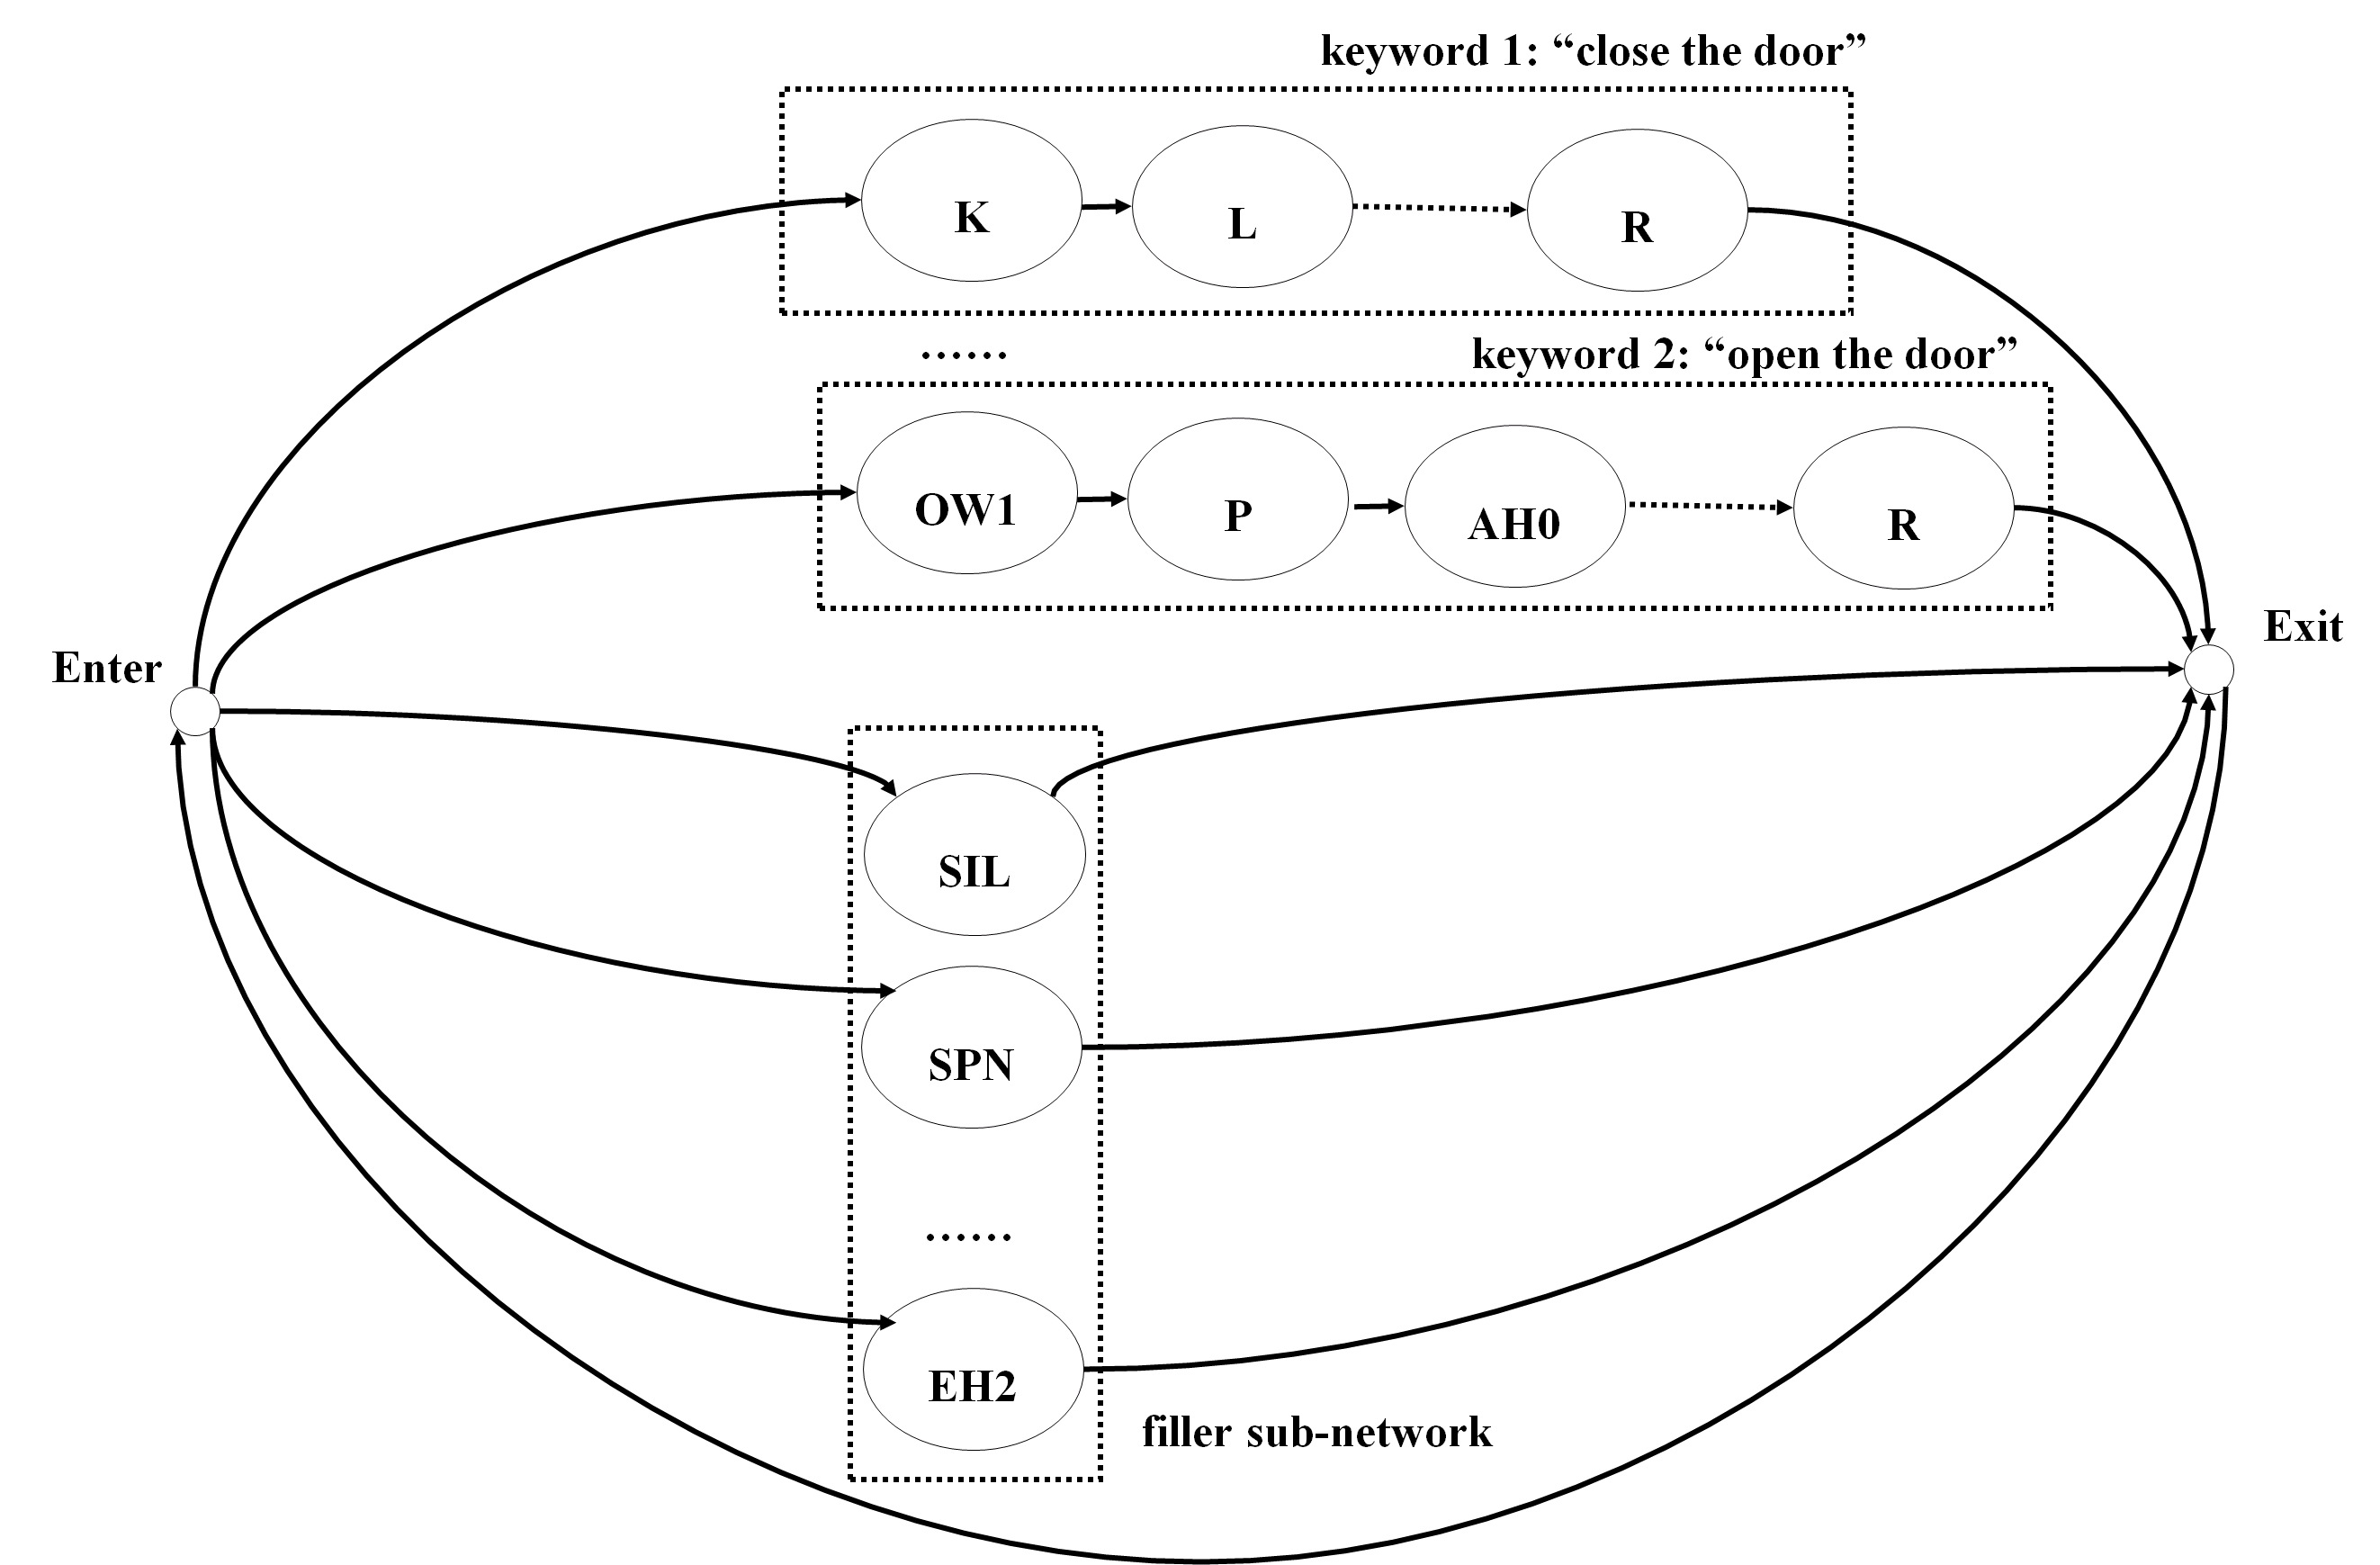
\includegraphics[width=\linewidth]{figure/filler-graph.png}
    \caption{\it 基于 $\tt filler$ 解码的搜索空间结构图}
    \label{fig:filler-graph}
\end{figure}

它包含了两个部分:领域内搜索空间和领域外搜索空间。前者由关键词的子序列建模得到,如图~\ref{fig:filler-graph}中的音素序列。 $\tt filler$ 子网络用于对领域外的搜索空间进行建模。$\tt filler$ 子网络是由所有的音素自环组成的。

\section{基于CTC的关键词检测的标签同步解码}
\label{Sec:kws-ctc}

\subsection{模型训练}
\label{Sec:modeltrain}

如前面章节\ref{Sec:sdm-sdt-intro}所述,序列鉴别性训练的关键之处是竞争序列的建模。
%criteria \& model unit
在本文中,我们研究了两种方向:词语建模和音素建模的CTC关键词检测模型。

为了更好地建模词级CTC模型的竞争序列,这里针对非关键词引入了新的建模单元。
类似于传统的声学KWS方法,代表非关键词的$\tt filler$被引入。在训练阶段, $\tt filler$ 则取代所有标注中的非关键词。

%word boundary modelling
另一个方向是针对音素级模型,我们进行修改的动机是:
i) 任何音素序列,也包括非关键部分,都可以由音素模型来进行建模。
ii) 使得声学模型容易做到与关键词无关,应用于非固定关键词的关键词检测任务。
%
除此之外,我们在词语边界处引入了 $\tt wb$ 单元~\cite{zhuang-is2016}。 在 音素 CTC 中 $\tt wb$ 和 $\tt blank$ 被分别作为词和音素的边界进行建模。区分这样的边界区段不仅可以改善泛化能力,而且也对后面将介绍的后处理有帮助。

这里针对引入的建模单元,公式修改如下:
\begin{equation}
\label{equ:ctc-kw}
\begin{split}
P(\mathbf{L}_u|\mathbf{O}_u)=P(\mathbf{L}_u'|\mathbf{O}_u)_{\mathbf{L}_u' = \mathcal{D}(\mathbf{L}_u)}
\end{split}
\end{equation}
$\mathcal{D}$ 是标签的映射函数。 $\mathcal{D}$ 针对词级或者音素级CTC具有不同的定义。
\begin{equation}
\label{equ:ctc-d}
\begin{split}
\mathcal{D}_{\tt{word}}:\mathbb{L}  \mapsto \mathbb{L}  \cup \{{\tt filler}\}\\
\mathcal{D}_{\tt{sub-word}}:\mathbb{L}  \mapsto \mathbb{L}  \cup \{{\tt wb}\}
\end{split}
\end{equation}
经过修改之后,在词级或者音素级建模中,搜索空间都将包含关键词,非关键词,音素边界和词边界。

\subsection{后处理}
\label{Sec:post-process-ctc}

我们进一步基于最小编辑距离(MED)提出了一个针对CTC推理分布的后处理方法,以便引入音素的混淆性先验知识,增强模型性能。这项工作受到\cite{chaudhari2007improvements}启发, 这里基于CTC词图和MED算法~\cite{7736093}l来针对音素引入混淆建模。 

%which generates a sub-word lattice on the basis of the output probability distribution of CTC and then performs search.  
图~\ref{fig:med-framework} 给出了在音素CTC中使用MED算法的框架。再一句音频中,关键词出现于CTC词图的概率是用三种编辑距离的概率相乘得到的,它们包括插入,删除,替换。每一种操作的概率由MED算法决定。现实中,每个音素在CTC的建模中性能可能各不相同,因此需要进一步采用音素的先验来设计每个音素的阈值,这部分可以通过预先统计得到~\cite{zhuang-is2016}。

\begin{figure}[htbp!]
\centering
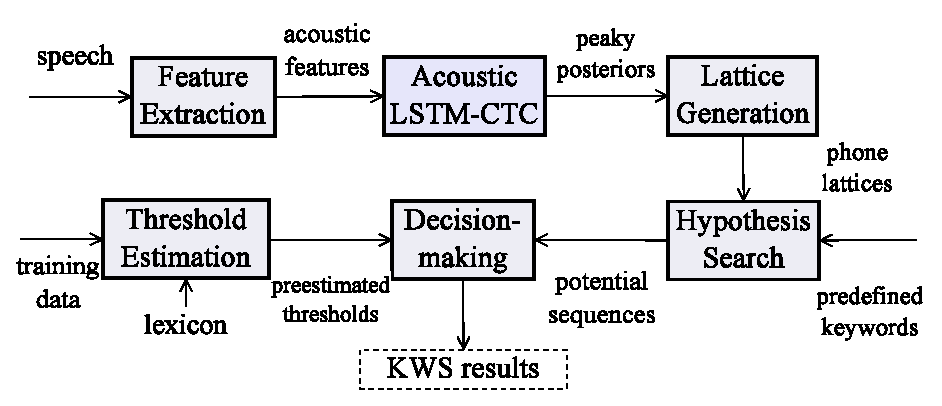
\includegraphics[width=\linewidth]{figure/kws-framework.eps}
\caption{\it 所提出的MED方法的框架。这里使用音素CTC作为例子}
\label{fig:med-framework}
\end{figure}

\subsection{序列鉴别性训练在HMM和CTC框架中的比较}
\label{Sec:disc-and-ctc}

本文中, 序列鉴别性训练被分为两种序列模型而进行: 生成式序列模型 和 鉴别式序列模型。在开始实验部分之前,我们先对两种做法进行一些综合比较:

\begin{itemize}
  \item {\em 生成和鉴别式序列模型}。 在HMM中,需要采用贝叶斯公式将序列状态转移概率和深度学习所估计的后验概率结合起来。在CTC中,给定特征序列后的标签序列的后验概率则直接由深度学习模型进行建模。
  \item {\em 序列建模}。 通过引入 $\tt{blank}$ 到每一帧分解后的建模当中,CTC隐性地对标签进行了序列建模。在HMM中,标签序列被显性地被N元语言模型进行限制和共同建模。
  在计算序列的后验概率时,两种框架都使用了前后向算法。
  \item {\em 混淆区段}. $\tt{blank}$ 原先是提供给CTC进行两个标签之间的混淆区段的建模的。类似的结构也可以如图~\ref{fig:hmm-topo}(c-e)所示在HMM中使用。除了拓扑结构的不同, $\tt blank$ 的粒度在HMM和 CTC中也是初始不同的。
  \item {\em 竞争序列建模}. 在词级CTC中,非关键词元素显示地由建模单元进行建模,即 $\tt filler$ 和 $\tt wb$。 在HMM中,我们采用音素单元对这些竞争序列进行隐性的建模。同时一个音素级的语言模型给出了音素搜索空间的建模效果。 %phone+explicit lm prior
  %\item {\em Discriminative training}. CTC directly models the sequence level posterior probability. The sequence discrimination is implied in the model. For GSM, 序列鉴别性训练 employs maximum a posteriori (MAP) criterion. The discrimination between the correct label sequence and competing hypotheses is modeled by the occupancy probability of the former versus that of the latter.
\end{itemize}

\section{实验结果}
\label{chap:kws-exp}

实验将分别在HMM和CTC框架下进行,我们对两种框架分别进行了序列鉴别性训练实验。
非固定关键词的关键词检测 (语料库检索 任务), 和固定关键词的关键词检测(唤醒词识别 任务)都在实验部分进行了考察。所有实验都是在声学KWS上进行。

%\subsection{非固定关键词的关键词检测 task}
%\label{Sec:}
\subsection{英文语料库检索任务}
\label{Sec:exp-sp-docu-detri}

\subsubsection{实验配置}
\label{Sec:exp-sp-docu-detri-setup}

Wall Street Journal (WSJ0)数据集的一个说话人独立的5k词表数据集 \cite{garofalo1993continous} 被用于评估基于 CTC词图的KWS。 至少出现过5词的词或短语被随机挑选出来作为关键词。总计有50个关键词。

由于WSJ0数据集比较小,同时关键词出现次数较少,因此我们在HMM和CTC中都使用音素作为建模单元,以提高泛化能力,而词作为建模单元将在下章中进行。
输出的音素由CMU 发音词典得到。24维对数filter-bank系数及其第一和第二阶导数组成了10ms固定帧率的特征序列。
HMM模型的配置与 \cite{povey2016purely}中相似,但使用了更好的参数如表~\ref{tab:model-discri} 和表 \ref{tab:perf-all}所示。 我们估计了三元的音素语言模型用于LF-MMI的训练。
%zhc00@qingdao:/aifs/users/zhc00/works/lfmmi/wsj/sjtu$ fstinfo exp/chain/tdnn_sjtu_mono_2n_mhmm1c.NSN.0.1.32.12_nd/phone_lm.fst
我们使用$\alpha=2.5$ 和 $\beta=2.5$ 作为 NU-LF-bMMI的参数。
CTC模型的配置详见 \cite{7736093}。我们使用单向 每层384节点的两层LSTM 进行实验,其带有 128 个节点的映射层。
%The LSTM network was initiated using cross-entropy criterion and then trained using CTC criterion.
%For performance comparison, conventional {\em keyword-filler} DNN-HMM was also trained as baselines. DNN has an 11-frame context window with 5 extended frames on the left and right. %Both HMM systems have 1689 clustered triphone states. 
所有声学模型都使用 Kaldi进行训练~\cite{povey2011kaldi}.
 {\em 等错误率} (EER) 用来度量上面两种测试下的错误率,该指标反映了无唤醒和未唤醒错误的均值。越低的EER表示越好的模型性能。
我们也绘出了receiver operating characteristic (ROC) 曲线,以总结实验结果。
在基于$\tt filler$ 的解码中, 表示为 {\em{kw-filler}}, 而EER是由扫描修改filler权重而得到的。
后验概率平滑,表示为 {\em{smooth}}, 和 CTC MED后处理方法, 表示为 {\em{MED}}, 都是通过\cite{7736093}中提出的固定阈值方法得到的。
\begin{equation}
\label{equ:eer-thres}
\begin{split}
\mathcal T_{EER}(\mathbf{k})=\mathcal T_0+\mathcal T(\mathbf{k})
\end{split}
\end{equation}
公式中 $\mathcal T(\mathbf{k})$ 是针对关键词 $\mathbf{k}$的阈值估计。 $\mathcal T_0$ 在所有关键词中共享,并通过调节它得到EER结果。

{\em 实时率} (RTF), 解码时间与音频时长的百分比, 被作为对整体速度的衡量指标。越低的RTF表示速度越好。
在测试阶段,我们使用的CPU型号为
{\em{Intel(R) Xeon(R) CPU E5-2690 v2 @ 3.00 GHz}}. 
%The ASR decoder used in kw-filler systems is an internal optimized WFST decoder. 
%Clustered cross-word tri-phone HMMs were used as baselines\footnote{Since the KWS task in this paper concerns unrestricted keyword vocabulary, keyword-specific approaches such as \cite{chen2014small} are not appropriate baselines.}.
%A GMM system with 40 Gaussian mixtures and a DNN system of 4 hidden layers with 512 nodes per layer were built.
%The acoustic feature for GMM is 13-dimensional cepstral mean normalized MFCC coefficients  with their first and second order derivatives.

\subsubsection{HMM和CTC模型训练}
\label{Sec:exp-model-arch}
\begin{itemize}
\item {生成式序列模型}
\end{itemize}

本章节比较了不同的声学模型配置。基于HMM的序列鉴别性训练结果见表~\ref{tab:model-discri}。
%model unit (context), hmm topo, MTL. 
这里的所有模型都是通过公式 (\ref{equ:kws-mmi})中的LF-MMI模型进行训练得到的,同时这里使用了KW-Filler的后处理方法。 
\begin{table}[thbp!]
  \caption{\label{tab:model-discri} {\it 基于HMM的序列鉴别性训练的模型框架}}
  %\vspace{1mm}
  \centerline{
    \begin{tabular}{c | c | c |c |c||c}
      \hline
      \multicolumn{1}{c|}{NN Model} &
      \multicolumn{1}{c|}{Context } &
      \multicolumn{1}{c|}{\# Param.} &
      \multicolumn{1}{c|}{CEW} &
      \multicolumn{1}{c||}{HMM} &
      \multicolumn{1}{c}{EER} \\
      \hline \hline
      \multirow{1}{0.1\columnwidth}{BLSTM}&\multirow{1}{0.05\columnwidth}{CD}& 0.60M & 0.1& \multirow{1}{0.05\columnwidth}{PB} & 3.3  
       \\
      \hline
      \hline
      \multirow{7}{0.1\columnwidth}{\textbf{TDNN}}&\multirow{1}{0.05\columnwidth}{CD} & 0.54M& 0.1&\multirow{1}{0.05\columnwidth}{PB}  & 3.3  
       \\
      \cline{2-6}
      &\multirow{6}{0.05\columnwidth}{\textbf{CI}}& \multirow{6}{0.1\columnwidth}{\textbf{0.51M}} & 0.1&\multirow{4}{0.05\columnwidth}{PB}  & 3.3  \\
      \cline{4-4}\cline{6-6}
      &&& 0.4&  & 3.2  \\
      \cline{4-4}\cline{6-6}
      &&&\textbf{0.7}& & 3.1  \\
      \cline{4-4}\cline{6-6}
      &&&1.0&& 3.2  \\
      \cline{4-5}\cline{6-6}
      &&&\multirow{2}{0.04\columnwidth}{0.7} &\multirow{1}{0.05\columnwidth}{\textbf{BP}}  & 3.0  \\
      \cline{5-5}\cline{6-6}
      &&&&\multirow{1}{0.05\columnwidth}{BPB}  & 3.0  \\
      \hline
    \end{tabular}
  }
\end{table}

我们首先对深度学习模型的架构进行了研究。第一二行比较了双向 LSTM (BLSTM) 和 时延神经网络(TDNN)在同等参数下的性能。 BLSTM 包含两层前后向各80个节点的LSTM网络。映射层包含30个节点。 CD TDNN 包含7层100个节点, CI TDNN 包含7层150个节点。结果显示了相似的EER性能。我们相信这是由于: i) 在KWS中,作为模型推理所需要的上下文并不需要很长,TDNN已经足够来针对这样的应用。 ii) 由于KWS模型的参数较少,因此限制了BLSTM模型的性能。在接下来的实验中,我们只讨论TDNN,原因是同等性能情况下它的速度更快~\footnote{我们暂未比较LSTM。近期的一些研究发现TDNN和LSTM可以被结合并取得更好的性能~\cite{tdnnlstm}}。
其次, 模型的建模单元在第二和三行中进行了比较。 tri-phone状态模型, 表示为上下文相关系统 (CD), 与单音素状态模型,表示为上下文无关系统 (CI)进行了比较。
CD模型基于三状态的从左到右的triphone 模型,包括 1536个绑定状态 (senones). 
%zhc00@qingdao:/aifs/users/zhc00/works/lfmmi/wsj/sjtu$ nnet3-info exp/nnet3/nnet_tdnn_a_tiny_smbr/final.mdl
它们的性能接近于 CI 模型。 %Besides the reason previously discussed, the stronger sequence level modeling effect in LF-MMI is another fold~\cite{povey2016purely}. 
第三,对于交叉熵规范化权重,表示为 CEW, 在第三到第六行中进行了调整。
结果显示 $0.7$ 可以得到最优结果,该值被使用在了后续的实验中。该值比LVCSR中偏大,原因是音素语言模型在测试阶段并不存在,这与LVCSR不同,因此训练过程仍在鉴别性训练和交叉熵准则之间权衡。
最终我们使用的拓扑结构如图~\ref{fig:hmm-topo} 
%
所示在第五,七和八行进行了比较。我们提出的BP,BPB比PB\cite{povey2016purely}轻微改善。 
但是在50个关键词上的显著性检验显示结果并不充分 ($\alpha=0.05$, $p=0.18$)。 
性能改善的原因可能为标签延迟所带来的改善~\cite{amodei2015deep},但需要后续更多的研究。 
%And the reason of the similar performance between BP and BPB is also that the label delay makes the confusion span of model inference,  B, mainly exist  before the label output, while the duration of certain pronunciation in the model unit is modeled by the self-loop in the label output HMM state,  P. 
由于BP的搜索空间比 BPB 小,而性能相似,因此后续实验使用BP。

\begin{table}[thbp!]
  \caption{\label{tab:criteria-discri} {\it 基于HMM的鉴别性训练的准则比较}}
  %\vspace{1mm}
  \centerline{
    \begin{tabular}{c ||c}
      \hline
      \multicolumn{1}{c||}{鉴别性训练准则 } &
      \multicolumn{1}{c}{EER} \\
      \hline \hline
%      CE& 4.0 \\
%      \hline\hline
%      CE+sMBR & 3.5 \\
%      \hline
      LF-MMI &3.0 \\
      \textbf{LF-bMMI} &2.9 \\
      LF-sMBR &2.9 \\
      \hline\hline
      NU-LF-bMMI &2.7 \\
      \hline
    \end{tabular} 
  }
\end{table}
第~\ref{Sec:lfmmi-train}章给出了不同准则,在表~\ref{tab:criteria-discri}中进行了比较。 % criteria: CE, mmi, b-mmi, smbr, NU-mmi. 
%The setup is as previously discussed, and 
这里使用 kw-filler进行后处理。 LF-bMMI 和 LF-sMBR 都显示好于 LF-MMI的性能,这与 LVCSR中的结论一致~\cite{vesely2013sequence}. 由于 LF-bMMI 训练快于 LF-sMBR 而性能相似,因此它被用在了后续实验中。
除此之外,NU-LF-bMMI 也参与了比较。这是一个固定关键词的关键词检测算法。在这种情况下,50个预先定义的关键词在训练阶段进行了使用,以加强关键词相关的梯度权重。经过训练之后,声学模型与关键词相关。
NU-LF-bMMI 带来额外的性能提升,而另一方面传统的固定关键词的关键词检测方法~\cite{chen2014small}并不能泛化这样的关键词无关训练集。后续NU-LF-bMMI 并不继续参与该数据集的比较,因为它与关键词无关算法并不可比。

%all tdnn CI kw-filler

\begin{itemize}
\item {鉴别式序列模型}
\end{itemize} 

在音素CTC中,引入的$\tt wb$ 建模单元在表~\ref{tab:wb}中进行了比较。对于少于6个音素的关键词被认为是短关键词,其余的为长关键词。因此可以将关键词集分成两部分分别检查他们的模型性能。
在短和长关键词中$\tt wb$都可以带来性能提升。长关键词的性能一致地优于短关键词,原因是短关键词的音素序列更可能是其他关键词的子集,造成了混淆和误唤醒率;$\tt wb$的引入缓解了这个问题。

 \begin{table}[h]
 \caption{\label{tab:wb} {\it 音素CTC在是否包含 $\tt wb$ 时的模型性能}}
  \centerline
  {
\begin{tabular}{cc||c}
\hline 
Keyword Length & wb & EER \tabularnewline
\hline 
\hline 
\multirow{2}*{short} & $\times$ & 9.0 \tabularnewline
& $\bm{\surd}$ & 4.5 \tabularnewline
\hline\hline
\multirow{2}*{long} & $\times$ & 3.1 \tabularnewline
 & $\bm{\surd}$ & 1.8 \tabularnewline
\hline 
\end{tabular}
 }
%\vspace{2mm}
\end{table}

\subsubsection{后处理和速度分析}
\label{Sec:exp-post-process}

不同的针对HMM和CTC的后处理算法在本节中进行了检查。值得注意的是,本部分是非固定关键词的关键词检测任务,因此音素被用来构建关键词序列。

\begin{table}[thbp!]
  \caption{\label{tab:post-discri} {\it  序列鉴别性训练系统的后处理}}
  %\vspace{1mm}
  \centerline{
    \begin{tabular}{c |c||cc}
      \hline
      \multicolumn{1}{c|}{Model (Crit.) } &
      \multicolumn{1}{c||}{Post} &
      \multicolumn{1}{c}{EER} &
      \multicolumn{1}{c}{RTF}\\
      \hline \hline
      HMM&  smooth &9.8&0.008 \\
      (LF-bMMI)& \textbf{kw-filler} &2.9&0.028\\
      \hline\hline
      %\multirow{2}{0.2\columnwidth}{NU-LF-bMMI}& smooth& 8.5  \\
      %& kw-filler&2.7\\
      %\hline\hline
      %0.026+0.012
       & smooth& 11.4  &0.026\\
     CTC & \textbf{kw-filler}&3.2&0.038\\
      & MED & 3.6 &0.031\\
      \hline
    \end{tabular}
  }
\end{table}
如表~\ref{tab:post-discri} 所示,在 LF-bMMI 和 CTC中,后验概率平滑方法会得到比 kw-filler显著差的结果。但是由于它的速度优势,该方法可以作为实际的前处理,滤除一些容易判断的样本,以减少语料库检索同的计算量。
在 CTC中我们比较了所提出的 MED 算法。
它显示了明显比kw-filler更差一些的性能,但效率较高。该方法将会在后续章节中进一步检验。
kw-filler系统可以使用前述的标签同步解码算法进行进一步速度优化,因此 CTC 可以得到比LF-bMMI更快的速度。最终系统CTC比LF-bMMI慢则源于其使用的LSTM速度比TDNN在LF-bMMI中的使用更慢。

\subsubsection{性能比较}
\label{Sec:exp-perf-comp}

最后,我们将性能和速度的比较总结在表~\ref{tab:perf-all}中。 同时我们绘制出了 ROC 曲线如图~\ref{fig:roc}, 其中越低的曲线结果越好。
其中所有的系统都使用kw-filler作为后处理方法。

\begin{table}[thbp!]
  \caption{\label{tab:perf-all} {\it  非固定关键词的关键词检测中的性能和速度比较}}
  %\vspace{1mm}
  \centerline{
    \begin{tabular}{c | c | c |c ||cc}
      \hline
      \multicolumn{1}{c|}{Model } &
      \multicolumn{1}{c|}{Context } &
      \multicolumn{1}{c|}{\# Param. } &
      \multicolumn{1}{c||}{Criterion} &
%      \multicolumn{1}{c||}{Post} &
      \multicolumn{1}{c}{EER} &
      \multicolumn{1}{c}{RTF} \\
      \hline \hline
      %\multirow{1}{0.05\columnwidth}{dnn}&\multirow{1}{0.05\columnwidth}{CD}&\multirow{1}{0.05\columnwidth}{2.0M}& CE & kw-filler & 5.1 & 0.074 \\
      %\hline
     &\multirow{1}{0.05\columnwidth}{CD}&\multirow{1}{0.05\columnwidth}{0.6M}& CE &  4.0 & 0.051 \\
      %0.015+0.036
      %\cline{2-7}
      %&\multirow{1}{0.05\columnwidth}{CI}&\multirow{1}{0.05\columnwidth}{0.5M}& CE & smooth & 10.2 & - \\
      %\hline \hline
       {TDNN HMM }&\multirow{1}{0.05\columnwidth}{CD}&\multirow{1}{0.05\columnwidth}{0.6M}& CE+sMBR & 3.5 & 0.050
       \\
       %0.015+0.036
       %\cline{2-7}
      &\multirow{1}{0.05\columnwidth}{CI}&\multirow{1}{0.05\columnwidth}{0.5M}& LF-bMMI &  \textbf{2.9} & \textbf{0.028}
       \\
       %0.008+0.020
       %\cline{4-7}
      %&&& NU-LF-bMMI & kw-filler & 2.7 & - \\
       \hline\hline
       \multirow{1}{*}{LSTM CTC}&\multirow{1}{0.05\columnwidth}{CI}&\multirow{1}{0.05\columnwidth}{0.8M}& CTC & \textbf{3.2} & \textbf{0.038} \\
      \hline
    \end{tabular}
  }
\end{table}

\begin{figure}
  \centering
    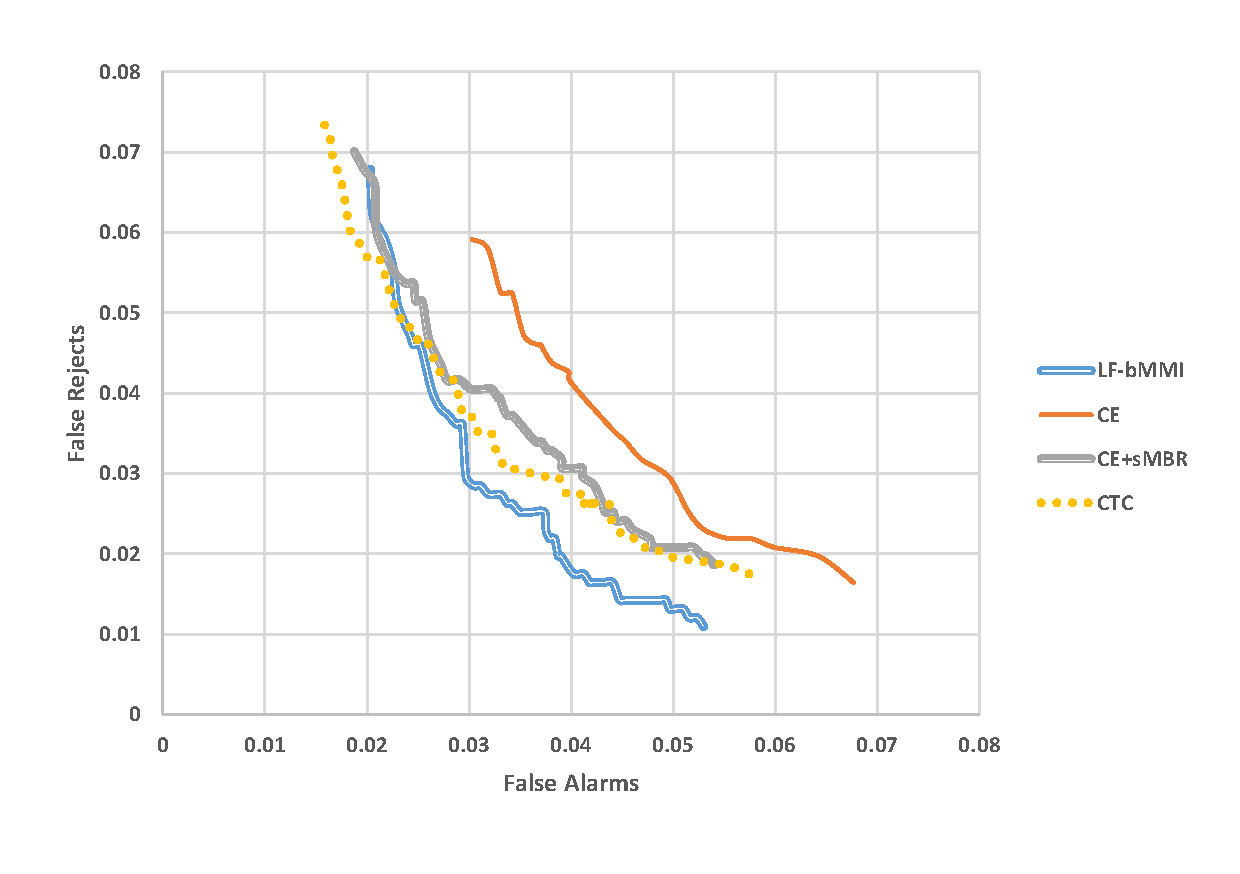
\includegraphics[width=\linewidth]{figure/roc.pdf}
    \caption{\it 非固定关键词的关键词检测的ROC 曲线比较}
    \label{fig:roc}
\end{figure}

这里我们使用交叉熵训练得到的系统作为第一行的基线。它是一个基于 NN-HMM 的传统系统,包含了聚类的tri-phone 状态建模。 这里的HMM拓扑结构见图~\ref{fig:hmm-topo}(a)。
传统鉴别性训练在交叉熵系统基础上进行。这里的词图由模型与一元语言模型解码得到~\cite{povey2007evaluation}。
前两行显示传统的词图鉴别性训练改善了 12\%性能,这一结论与LVCSR中类似~\cite{povey2005discriminative}。 在RTF上的轻微改善则是由于更好的声学模型提供了更少的搜索混淆性。

第三行对比第二行显示了所提出的最好的基于HMM的序列鉴别性训练方法与传统鉴别性训练方法的比较。
%Result shows two folds of superiority
这里显示出 17\% 相对改善 ($\alpha = 0.05$, $p = 0.06$, 在显著性检验测试中) 相比传统鉴别性训练和 28\% 相对改善 ($\alpha = 0.05$, $p = 10^{-5}$)  相比交叉熵训练系统。
这来源于更好的在所提出方法中的建模效果:
\begin{itemize}
 \item 如前文所述,修改后的HMM结构和更低的帧率都能带来性能的改善。
 \item KWS模型的LVCSR词图并不包含较好的竞争路径。这些词图来自声学模型与语言模型的共同解码,而KWS的声学模型性能较弱,并不是针对ASR识别进行设计的。因此这些质量更差的词图限制了鉴别性训练所带来的提升。
 \item 传统鉴别性训练在生成词图时候使用的词级别语言模型在KWS的测试阶段并不存在。而LF-MMI中使用的词级别语言模型则是对于测试阶段使用的由词典构成的关键词序列的一个很好的近似。
\end{itemize}
除此之外,与CE基线相比,LF-bMMI 系统取得了一倍的加速,原因在于模型推理和解码搜索都得到了加速。对于前者,主要是由于帧率减少。而后者主要是由于所使用的CI单元比传统CD单元少,使得搜索空间变少,这也包括对filler模型的相应简化。

使用LSTM的CTC系统在最后一行中,也显示了比传统CE模型更好的性能 ($\alpha = 0.05$, $p = 0.01$) 以及比传统鉴别性训练系统更好的性能 ($\alpha = 0.05$, $p = 0.11$)。 从图~\ref{fig:roc}中看, CTC系统存在相对较多误唤醒。

我们在一些初始的尝试中使用基于HMM的序列鉴别性训练作用在CTC初始化的变种模型上~\cite{sak2015fast,nict-icassp17}。但结果并不成功,没有带来改善: 在词级别CTC中~\cite{li2018developing}, LVCSR 解码词图不包含有效的竞争路径 。而在音素级别模型上,如前所述,词图的质量限制了传统框架下鉴别性训练所能得到的改善。% ii) Essentially, after CTC pre-training, the state prior probability $P(\mathbf{L})$~\cite{nict-icassp17} is combined with the original model to form a CTC variant. The CTC variant models $P(\mathbf{O}|\mathbf{L})$, and become a GSM. 

\subsection{中文数据集唤醒词识别}
\label{Sec:exp-wakeup-word-rec}
\subsubsection{实验配置}
\label{Sec:exp-wakeup-word-rec-setup}
%data
%20170321 bj123 定制唤醒词 baseline.txt
本章节进一步测试了在固定关键词的KWS系统中的性能。我们准备了一个类似于文献\cite{chen2014small}和  \cite{cas-icassp17}中介绍的数据集。它包含两部分:通用语音数据和关键词相关数据集。第一部分包含100小时,第二部分包含30K关键词正例,和180K关键词负例。详细的数据集配置可以参见~\cite{chen2018kws}。

%metrics
测试数据包含两部分:关键词相关集合和环境噪声集合。第一部分用于测试模型在区分关键词和非关键词时候的能力\cite{chen2014small}。 它们包含2K正例和10K负例,代表了 20\% 左右的比值,这符合该应用的实际应用场景。前文我们讨论的EER被作为准则。
环境噪声集合则用于测试模型对误唤醒的鲁棒性\cite{cas-icassp17}。它包含300小时的环境噪声。每小时的误唤醒次数记为 {\em{误唤醒频率}} (FAF), 也被作为度量模型性能的指标。
后处理中获取EER的超参数方法如前面章节所述。
每个关键词都单独包含它自己专门的平滑方法的阈值。总体的EER是每个关键词EER的平均值。
之后我们会固定所有的超参数并测试系统在噪声集合中的FAF。

%model 
在该任务中,我们测试了词级系统和音素级系统。HMM和CTC的鉴别性训练系统与传统交叉熵系统进行了比较。词级系统的输出为关键词序列中的每个词,而音素级系统的输出则为中文中的不带调音节。特征和声学模型配置与前面章节一致。
NU-LF-bMMI采用$\alpha=10.0$ 和 $\beta=10.0$。

\subsubsection{实验结果和比较}
\label{Sec:exp-wakeup-word-rec-result}

表~\ref{tab:perf-mandarin}显示了相应的结果。
一个交叉熵训练的词级别的TDNN系统被作为基线系统~\cite{chen2014small}。该系统采用了后验平滑作为后处理方式。

%compare EER \& FAF

\begin{table}[thbp!]
  \caption{\label{tab:perf-mandarin} {\it  固定关键词的KWS系统的性能和速度比较}}
  %\vspace{1mm}
  \centerline{
    \begin{tabular}{c|m{4.5em}|c|c||ccc}
      \hline
      %&
      %&&& \multicolumn{4}{c}{post-processing} \\
      %\cline{4-7}
      %&
      %&&&  \multicolumn{2}{c}{smooth} & \multicolumn{2}{c}{kw-filler} %& \multicolumn{2}{c}{MED}\\
      %\cline{4-7}
      \multicolumn{1}{c|}{Model}
      &\multicolumn{1}{c|}{Unit} 
      &\multicolumn{1}{c|}{Criterion}&\multicolumn{1}{c||}{Post }&EER&FAF&RTF%&FS&RTF
      \\
      \hline\hline
      %/aifs/users/zhc00/works/kws/lfmmi_chn700/exp/nnet3/chn700.subsetby20_train.nnet_tdnn_a_tiny/
      \cite{chen2014small}
      &\multirow{1}{*}{Word}
      &CE &smooth & 6.2 & 0.64 &0.014\\
      %0.013
     \hline\hline
      %
      \multirow{3}{*}{HMM}&\multirow{3}{*}{Syllable}
      &CE & & 10.2 & 1.40 &0.041\\
      %0.015+0.026
      %\cline{3-7}
      %/aifs/users/zhc00/works/kws/lfmmi_chn700/exp/chain/.tdnn_sjtu_mono_2n_mhmm1c.0.1.128.4_nd.chn700/
      && LF-bMMI &kw-filler &8.3& 1.06 &0.033\\
      %0.008+0.025
      %\cline{3-7}
      %/aifs/users/zhc00/works/kws/lfmmi_chn700/exp/chain/res_a.0.99.tdnn_sjtu_mono_2n_mhmm1c.0.1.128.4_nd.chn700/decode_testset.full.lnovopc_mcsnor_evl17feb_v1_graph_res3/scoring_kaldi/kws.rst2
      %exp/chain/chn700.subsetby5_train.res_a.0.99.tdnn_sjtu_mono_2n_mhmm1c.0.1.128.4_nd.chn700/decode_testset.full.lnovopc_mcsnor_evl17feb_v1_graph_res3/scoring_kaldi/kws.rst2
      && NU-LF-bMMI& & \textbf{5.2} &\textbf{0.51} &\textbf{0.029}\\
      %0.008+0.021
      \hline\hline
      %/aifs/users/zhc00/works/kws/ctc_chn700/ctc
      \multirow{2}{*}{CTC}
      &\multirow{1}{*}{Word}
      & \multirow{2}{*}{CTC} &smooth &9.1 & 1.13 & 0.024  \\
      %\cline{2-2}\cline{4-7}
      %ref: https://spetechcular.com/trac/asr/wiki/ctc_kws_chn_car https://spetechcular.com/trac/asr/wiki/%E6%AF%85%E8%90%8C2016#a2016.6.6
      &\ +{\tt filler}& &MED & \textbf{7.0}&\textbf{0.90} & \textbf{0.029}\\
      %0.024
      \hline
    \end{tabular}
  }
\end{table}

在第二行中,模型也是通过CE准则进行训练的。模型的建模单元是音节,后处理方法为 kw-filler。 
该系统性能在EER和FAF中都有所下降,原因是音素级系统具有更多建模单元。而这些建模单元都被等同地进行训练。与之相反,词级系统则可以对特定关键词具有更强的建模能力。
\cite{chen2014small}中显示了类似结论,这说明后验概率平滑方法的CE模型系统是一个较强的基线系统。

在第三行中,我们所提出的LF-bMMI系统显著改善了CE系统,取得了一致更优的EER和FAF。但是,所得到的系统仍然差于基线系统。为了解决针对关键词区段识别性能差的问题,我们使用了NU-LF-bMMI 方法,在第四行中。结果显示NU-LF-bMMI 系统得到了相对第一行基线中显著更好的结果。我们认为这包括两方面原因:第一,非一致地训练关键词相关的音素序列,理论上等同于对关键词的每个词单元专门进行训练,所以其建模能力类似; 第二,由于音素系统通过所提出的NU-LF-bMMI增强了关键词之间与关键词和非关键词之间的鉴别能力,因此它能够取得更优的性能。关于效率,虽然该系统的模型推理速度较快,但由于引入kw-filler的搜索部分,因此导致两倍的速度减慢。使用标签同步解码算法对系统进行加速是未来一个值得研究的问题。

最终,CTC系统也参与了比较。在第五行中的系统类似于\cite{fernandez2007application}。虽然它在文献\cite{fernandez2007application}中取得了较好的性能, 但在本部分测试中仍然差于词级别的CE系统。我们相信这是因为我们使用的训练和测试集相比该文献具有更大的挑战。我们针对这一系统如前文所述,添加了 $\tt filler$ 建模单元,以改善关键词与非关键词之间的鉴别性;同时我们增加了基于 MED的后处理算法,以便引入音素混淆性的先验知识。我们所提出的系统在第六行中取得了显著更好的结果。但是这个系统仍然没有超过传统的CE系统。
%This may be because the baseline in fixed vocabulary KWS is highly tuned while the CTC-MED approach treats all phones equally during training. It is worth noting that due to the same reason, the LF-bMMI approach does not outperform the baseline neither. 
我们认为进一步的改善应该包括两方面:对CTC模型的噪声鲁棒性的研究;使用更好的深度学习模型来改善模型性能。
%in keyword specific corpus 

%MED uses


\section{本章小结}
\label{chap:kws-sum}

本章节提出了基于序列鉴别性训练的深度学习关键词检测模型的训练框架。通过使用音素语言模型或者使用显性添加建模单元的方式,对竞争可能路径进行建模,由此得到更好和更快的序列鉴别性训练。
我们的实验在语料库检索任务和唤醒词识别任务上进行。对于前者,词表大小通常是无限制的,而对于后者,则要求有更强的噪声鲁棒性。尽管不同应用具有不同的特征,但是实验显示我们所提出的鉴别性训练方案可以取得一致和显著的改善,相比于传统的逐帧CE深度学习模型在固定关键词和非固定关键词的关键词检测任务上的最好的系统。
